\chapter{Introducción}


\begin{wrapfigure}{r}{.5\textwidth}
    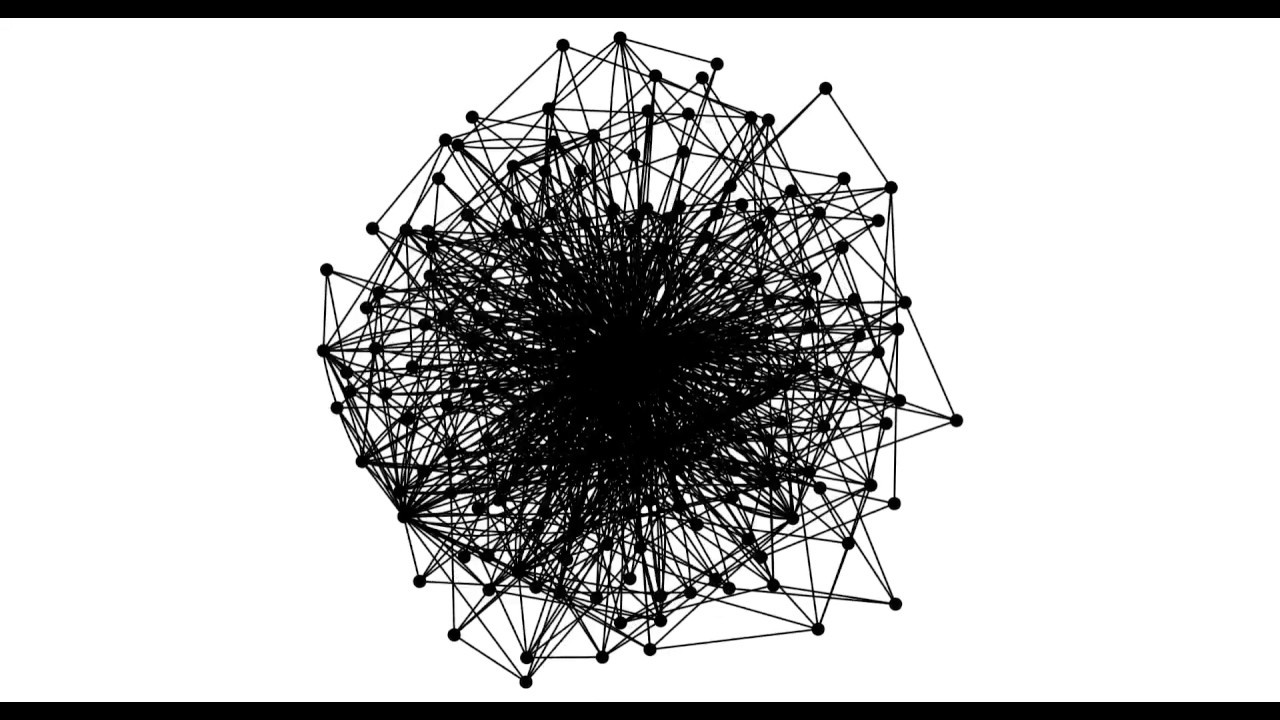
\includegraphics[width=.5\textwidth]{Tesis/Figures/smallworld.jpg}
    \caption{Gráfica del mundo pequeño con 500 nodos}
\end{wrapfigure}

Los grafos son objetos compuestos de cosas y las relaciones entre ellas. Los nodos de un grafo representan entidades mientras que las aristas son cualquier tipo de interacción o conexión entre las entidades. Existen una variedad de tipos de grafos, desde grafos sociales, grafos de colaboración, grafos financieros y muchos más. Las representaciones visuales de los grafos tienden a ser un poco confusas pues sólo son líneas conectando círculos y conforme crece el número de elementos se vuelven aún más confusas.

Sin embargo, sabemos que las interacciones entre las entidades, sean personas o bancos, rara vez se dan de forma aleatoria. Las motivaciones para la creación de una relación entre entidades no puede observarse directamente a partir de las aristas en un grafo ni tampoco se pueden deducir ojeando la base de datos que contenga los datos relacionales. Sin embargo, en nuestro repertorio de herramientas se encuentran diversas técnicas de análisis matemático que nos permiten hacer un análisis más completo de los grafos. En esta tesis se va a plantear el marco teórico de los modelos de grafos aleatorios exponenciales (ERGMs) que son un tipo de regresión logística modificada que permiten calcular la probabilidad de que exista una arista dado la presencia de otras aristas dentro de un grafo.


\section{Antecedentes}

Las grafos sociales impregnan nuestra vida social y económica pues juegan un papel central en comunicar oportunidades de trabajo, estatus social, información sobre el mundo y son críticas para el funcionamiento del mundo digital. Las grafos sociales también son importantes para predecir cómo se esparcen las enfermedades, qué productos son populares, qué lenguas se hablan y además repercuten en la forma en la que participamos en nuestras democracias. Es por todas estas razones que si queremos entender el mundo y hacerlo más próspero debemos de entender las estructuras fundamentales de las grafos y de qué forma se presentan en nuestra sociedad.

El propósito de esta tesis es proporcionar un marco teórico para el análisis de las grafos manteniendo en mente el importante aspecto social.

Por mucho tiempo ha sido de interés para los matemáticos encontrar formas para describir las características de una red observada. Estas grafos se han presentando en nuestras estructuras sociales desde el inicio del tiempo sea a través de las grafos sociales de amigos, las grafos de comercio, las grafos de influencia y muchas otras más. En particular desde la apertura del internet, que conlleva el registro de nuestras actividades humanas en bases de datos digitales, la disponibilidad de bases de datos de estas grafos se ha disparado.

Las actividades de usuarios en internet pueden ser registradas con gran detalle. Este monitoreo está presente a través de casi todas las plataformas que crean contenido y existen un gran número de distintas implementaciones para monitorear el comportamiento de los usuarios en estas mismas plataformas. A través del tiempo las empresas han acumulado mucha información sobre sus usuarios con la meta de comprender a sus audiencias. Por ejemplo, si un usuario a menudo consume cierto tipo de contenido entonces este mismo usuario es más probable que esté interesado en ese tipo de contenido en el futuro. Entonces, al monitorear las actividades de los usuarios es que se puede crear una representación del tipo de contenido consumido por los usuarios y se pueden generar modelos para recomendarle contenido relevante a todos.


Grandes empresas han dedicado muchos recursos al modelaje del comportamiento de sus usuarios como Facebook, Linkedin, Netflix y Amazon. Sin embargo, la información recopilada de los usuarios de una sola plataforma puede estar sesgada pues los usuarios en realidad pueden consumir distintos tipos de contenido de distintas páginas. Sin embargo, existen varias soluciones a este problema de seguir a los usuarios en las distintas plataformas en las que consumen contenido. Para conseguir una mejor representación de las preferencias de un usuario cualquiera se han utilizado \textit{cookies} anónimas en donde la tecnología de sincronización juega un rol esencial. Esta tecnología permite el rastreo de las acciones registradas en un buscador de internet.

Cuando un usuario visita un sitio el proveedor del contenido genera una \textit{cookie} que está atada al buscador del usuario. Entonces, el proveedor de contenido \textit{hashea} la clave del usuario y la registra en una base de datos de un proveedor de servicios estratégicos, como un \textit{Data Management Platform (DMP)}. Además en ese mismo momento se registra el tipo de comportamiento del usuario en una base de datos y el usuario se le asigna una audiencia en un mercado de audiencias en el cual cualquier tercero puede añadir esos usuarios anónimos a sus audiencias. Los terceros por su parte se comprometen a registrar el comportamiento de los usuarios de sus propiedades digitales y lo suben a la misma base. Las empresas pueden también utilizar sus bases de datos \textit{offline}, como el registro de compras de un \textit{ecommerce}  y asignarle una clave única a cada usuario para después cruzar los datos \textit{offline} con los comportamientos registrados en línea. A esto se le conoce como \textit{cookie syncing} y permite atar los datos que se generan en línea con aquellos que se registran a nivel físico y comercial.

Las empresas pueden generar enormes conocimientos sobre sus usuarios a partir de este tipo de prácticas de recolección de datos. De hecho existen casos extremos en donde las empresas a partir del perfil de consumidor que generaron de sus clientes pueden predecir cosas sobre sus clientes antes que ellos mismos. Un caso pronunciado de esto fue cuando un padre se entero que su hija estaba embarazada por \textit{Target} antes de que ella misma supiera. 

Estas bases de datos de usuarios anónimos son particularmente valiosas para los departamentos de marketing en las empresas y su venta representa una importante fuente de ingresos para las empresas que generan información sobre sus usuarios. Estas bases de datos de terceros permiten la implementación de la publicidad dirigida que se ha vuelto cotidiana en nuestra navegación en internet.

\section{Filtros Colaborativos}

Una de las implementaciones de modelos más famosas y útiles que han utilizado las bases de grafos se les conoce como filtros colaborativos. La idea esencial detrás de este modelo es que podemos utilizar las preferencias de usuarios parecidos entre sí para recomendar contenido. Es decir que utilizamos la información sobre miembros parecidos para hacer inferencias sobre un consumidor cualquiera.

Uno de los casos más exitosos y uno de los más personalmente importantes para mí es aquel de \textit{Spotify}, en donde se utilizan los filtros colaborativos para darle vida a uno de los principales diferenciadores de la empresa en el competitivo ámbito del \textit{streaming} de música: \textit{Spotify weekly}. La idea principal de lo que se hace en \textit{Spotify} viene ilustrada en la siguientes páginas. La idea es simple, si muchos usuarios escuchan las canciones $x,y,z$ entonces esas canciones probablemente son similares. Además si muchos usuarios escuchan las canciones $x,y,z$ y un usuario escucha las canciones $x$ y $y$ entonces deberíamos de recomendarle escuchar la canción $z$.

Todo empieza con el registro de todos los usuarios de \textit{Spotify} en donde cada usuario $u_j$ tiene asignadas las canciones $i_j$ que escuchó a un momento $t_k$:

$$\begin{array} { l } { \left( u _ { 1 } , i _ { 1 } , t _ { k } \right) } \\ { \left( u _ { 2 } , i _ { 2 } , t _ { k } \right) } \\ { \cdots } \\ { \left( u _ { n } , i _ { n } , t _ { k } \right) } \end{array}$$

Sin embargo esta representación es un poco difícil de interpretar, entonces lo que se hace es que se agregan los datos y expresamos los datos temporales en una matriz pues no importa si es que el usuario escuchó una canción una vez hace una semana y 11 veces ayer o si la escuchó 12 veces ayer si queremos saber cuáles canciones escuchó en la semana. Entonces se pueden representar todos los datos en una matriz de la siguiente forma:


$$N = \underbrace { \left( \begin{array} { c c c c } { c _ { 11 } } & { c _ { 12 } } & { \dots } & { c _ { 1 n } } \\ { c _ { 21 } } & { c _ { 22 } } & { \dots } & { c _ { 2 n } } \\ { \vdots } & { } & { } & { \vdots } \\ { c _ { m 1 } } & { c _ { m 2 } } & { \dots } & { c _ { m n } } \end{array} \right) } _ { \text {Canciones en Spotify } } \} \text { Usuarios en Spotify}$$



En esta matriz cada renglón representa un usuario y cada columna representa una canción en la biblioteca de \textit{Spotify}. Los elementos de la matriz $c_{ ij }$ son números enteros que representan la cantidad de veces que el usuario i escuchó la canción j. Esta gigantesca matriz con alrededor de $10^7 \times 10^7$ elementos tiene muchos problemas además de su enorme tamaño pues tiene muchos elementos iguales a cero (que dificultan el aprendizaje no supervisado) y muchos elementos desconocidos en caso de que se use para un problema de aprendizaje supervisado y además en realidad no necesariamente representa información verídica sobre los gustos de las personas pues las personas pueden escuchar canciones en modo \textit{offline} o de otras personas. En general es bastante difícil trabajar con esta matriz, afortunadamente los matemáticos en \textit{Spotify} son capaces de encontrar muchas formas de extraerle significado.

Por ejemplo se puede llevar a cabo el análisis entre columnas utilizando una medida de correlación como Pearson para ver qué tan similares son las columnas como en

$$c _ { i j } = \frac { \sum _ { u } N _ { u i } N _ { u j } } { \sqrt { \sum _ { u } N _ { u i } ^ { 2 } } \sqrt { \sum _ { u } N _ { u j } ^ { 2 } } }.$$

De hecho es así como \textit{Amazon} arroja las recomendaciones de productos cuando nos dice que los ``usuarios que compraron esto también compraron…''. Sin embargo la paralelización de esto es difícil pues el numerador en esa expresión es bastante denso aún cuando se tienen matrices pequeñas como

$$N = \left( \begin{array} { c c c c } { 0 } & { 7 } & { 21 } & { 0 } \\ { 5 } & { 0 } & { 0 } & { 1 } \\ { 4 } & { 0 } & { 13 } & { 9 } \\ { 0 } & { 0 } & { 0 } & { 7 } \\ { 19 } & { 1 } & { 0 } & { 13 } \\ { 0 } & { 3 } & { 0 } & { 0 } \end{array} \right)$$

En donde tendríamos que calcular 

$$N ^ { T } N = \left( \begin{array} { c c c c } { 402 } & { 19 } & { 52 } & { 288 } \\ { 19 } & { 59 } & { 147 } & { 13 } \\ { 52 } & { 147 } & { 610 } & { 117 } \\ { 288 } & { 13 } & { 117 } & { 300 } \end{array} \right)$$


Para calcular la correlación entre usuario o canciones.

Existen otras formas para utilizar esta matriz de forma más conveniente, por ejemplo lo que se llama \textit{Probabilistic Latent Semantic Analysis (PLSA)} en donde la idea es que queremos calcular las probabilidades del siguiente evento descomponiendo la matriz de tal forma que tengamos vectores de usuarios y vectores de canciones. Este es el algoritmo que de hecho se implementó dentro de \textit{Spotify} pero su explicación a detalle está fuera del alcance de esta tesis.

Fue en el transcurso de aprender más sobre la implementación de los distintos algoritmos de recomendación que empecé a trabajar en Hexagon Data, una empresa que se dedica al marketing digital, donde se me abrieron las puertas a una enorme base de datos en donde se registraban el 1\% de todas las actividades en internet. Con esta base de datos en mis manos y con las ganas de innovar es que decidí enfrentar el problema de la recomendación para descubrir conglomerados de contenido y generar audiencias de forma automatizada.


\section{Objetivo}

El objetivo de esta tesis es describir y proveer un marco teórico para el modelaje de grafos, la exploración de los modelos exponenciales, la introducción a las grafos aleatorias exponenciales, describir a las grafos sociales a través de estadísticas y proponer la implementación de un modelo de grafos aleatorias exponenciales para la utilización en la predicción del estado futuro de una red de preferencias entre usuarios y contenido a partir de la estadísticas extraídas de sus características. 


\section{Alcance}

Los modelos aleatorios de grafos exponenciales resultan bastante útiles en la descripción de las grafos sociales pues se extraen los valores de los parámetros a estimar que pueden estar asociadas a triadas u otras medidas cuya naturaleza depende de la interacción entre los nodos de la red. Es decir que el modelo permite incorporar elementos de probabilidad condicional cuando se hace la predicción del futuro de la red. Esto es consistente con el razonamiento que las personas que están interesadas en algún tipo de contenido en particular son más propensas a estar interesadas en ese tipo de contenido en el futuro. De otra forma es que si muchas personas hacen $x, y$ y $z$, entonces $x, y$ y $z$ son probablemente similares. También se puede esperar que los subgrafos de nodos que están altamente conectados seguirán estando conectados en el futuro.

Existen muchas preguntas respecto al análisis de grafos sociales que tienen que ver con el enigma de cómo es que procesos y estructuras sociales locales contribuyen a la estructura global de un grafo y si es que estos procesos locales son suficientes para explicar las preguntas que tenemos de nuestro modelo. Las realizaciones que resultan de las combinaciones de muchos procesos locales no son generalmente intuitivas, ni siquiera de forma cuantitativa. 

Posiblemente podemos navegar estos difíciles problemas con el uso de la simulación. Sin embargo, es importante tener en mente que nuestra observación de un grafo en realidad es únicamente una posible configuración de un conjunto de posibles grafos que tienen  características similares y, aunque el número de actores sea conocido, en realidad es el producto de un proceso estocástico desconocido.

Es justo nuestro enorme interés en registrar las interacciones entre los actores lo que hace la estimación de la red en el futuro particularmente difícil. Esto es porque las relaciones generalmente no son independientes y sólo podemos observar a la Grafo en un momento en el tiempo (un momento antes del futuro) y como veremos más adelante los estimadores de máxima verosimilitud de las grafos exponenciales muchas veces son desconocidos y aunque no lo fueran es computacionalmente demandante trabajar con ellos. Como veremos más adelante se utilizarán los estimadores de máxima pseudo verosimilitud que se obtienen a través del cálculo de las probabilidades condicionales completas. El teorema de Hammersley-Clifford que será demostrado más adelante forma los cimientos del marco teórico en el cual esta tesis se basa.

Los modelos de grafos exponenciales aleatorias intentan contestar al tipo de preguntas incómodas como ¿Es más probable que la gente se asocie con los amigos de sus amigos? ¿Las personas son menos propensas a asociarse con personas de distintas clases sociales? Estas preguntas se pueden intentar contestar a partir de las estructuras sociales que conforman nuestras vidas. Estos modelos generan conclusiones sobre nuestras formas de aprendizaje, la desigualdad, la propensidad a la innovación de distintas estructuras sociales y mucho más.
